%\section{Introduction}

\section{Motivation}

\subsection{Web application cluster}

Today, a great number of people in the world can not spend a day without using smartphones or personal computers(PCs) to retrieve information from the Internet for work or for daily life.
For example, people use these devices to look up web pages, emails, social media and sometimes to play games.
These services are often called web applications or web services, where information is delivered using Hyper Text Transfer Protocols(HTTP) or Hypertext Transfer Protocol Secure (HTTPS) from servers at the other end of the Internet.
Web applications are provided by various organizations, including commercial companies, government, non-profitable organizations, etc.

For example, Google provides a variety of web services including, Gmail, Search engine, Google Suits, etc.
Facebook provides social media service, Amazon provides shopping sites.
Governments provides information regarding the service they provide to their citizens.
Schools often provide a syllabus to their students, which is important for campus life.
The author calls those organizations that provide web applications, web application providers hereafter.

\begin{figure}[h]
\begin{center}
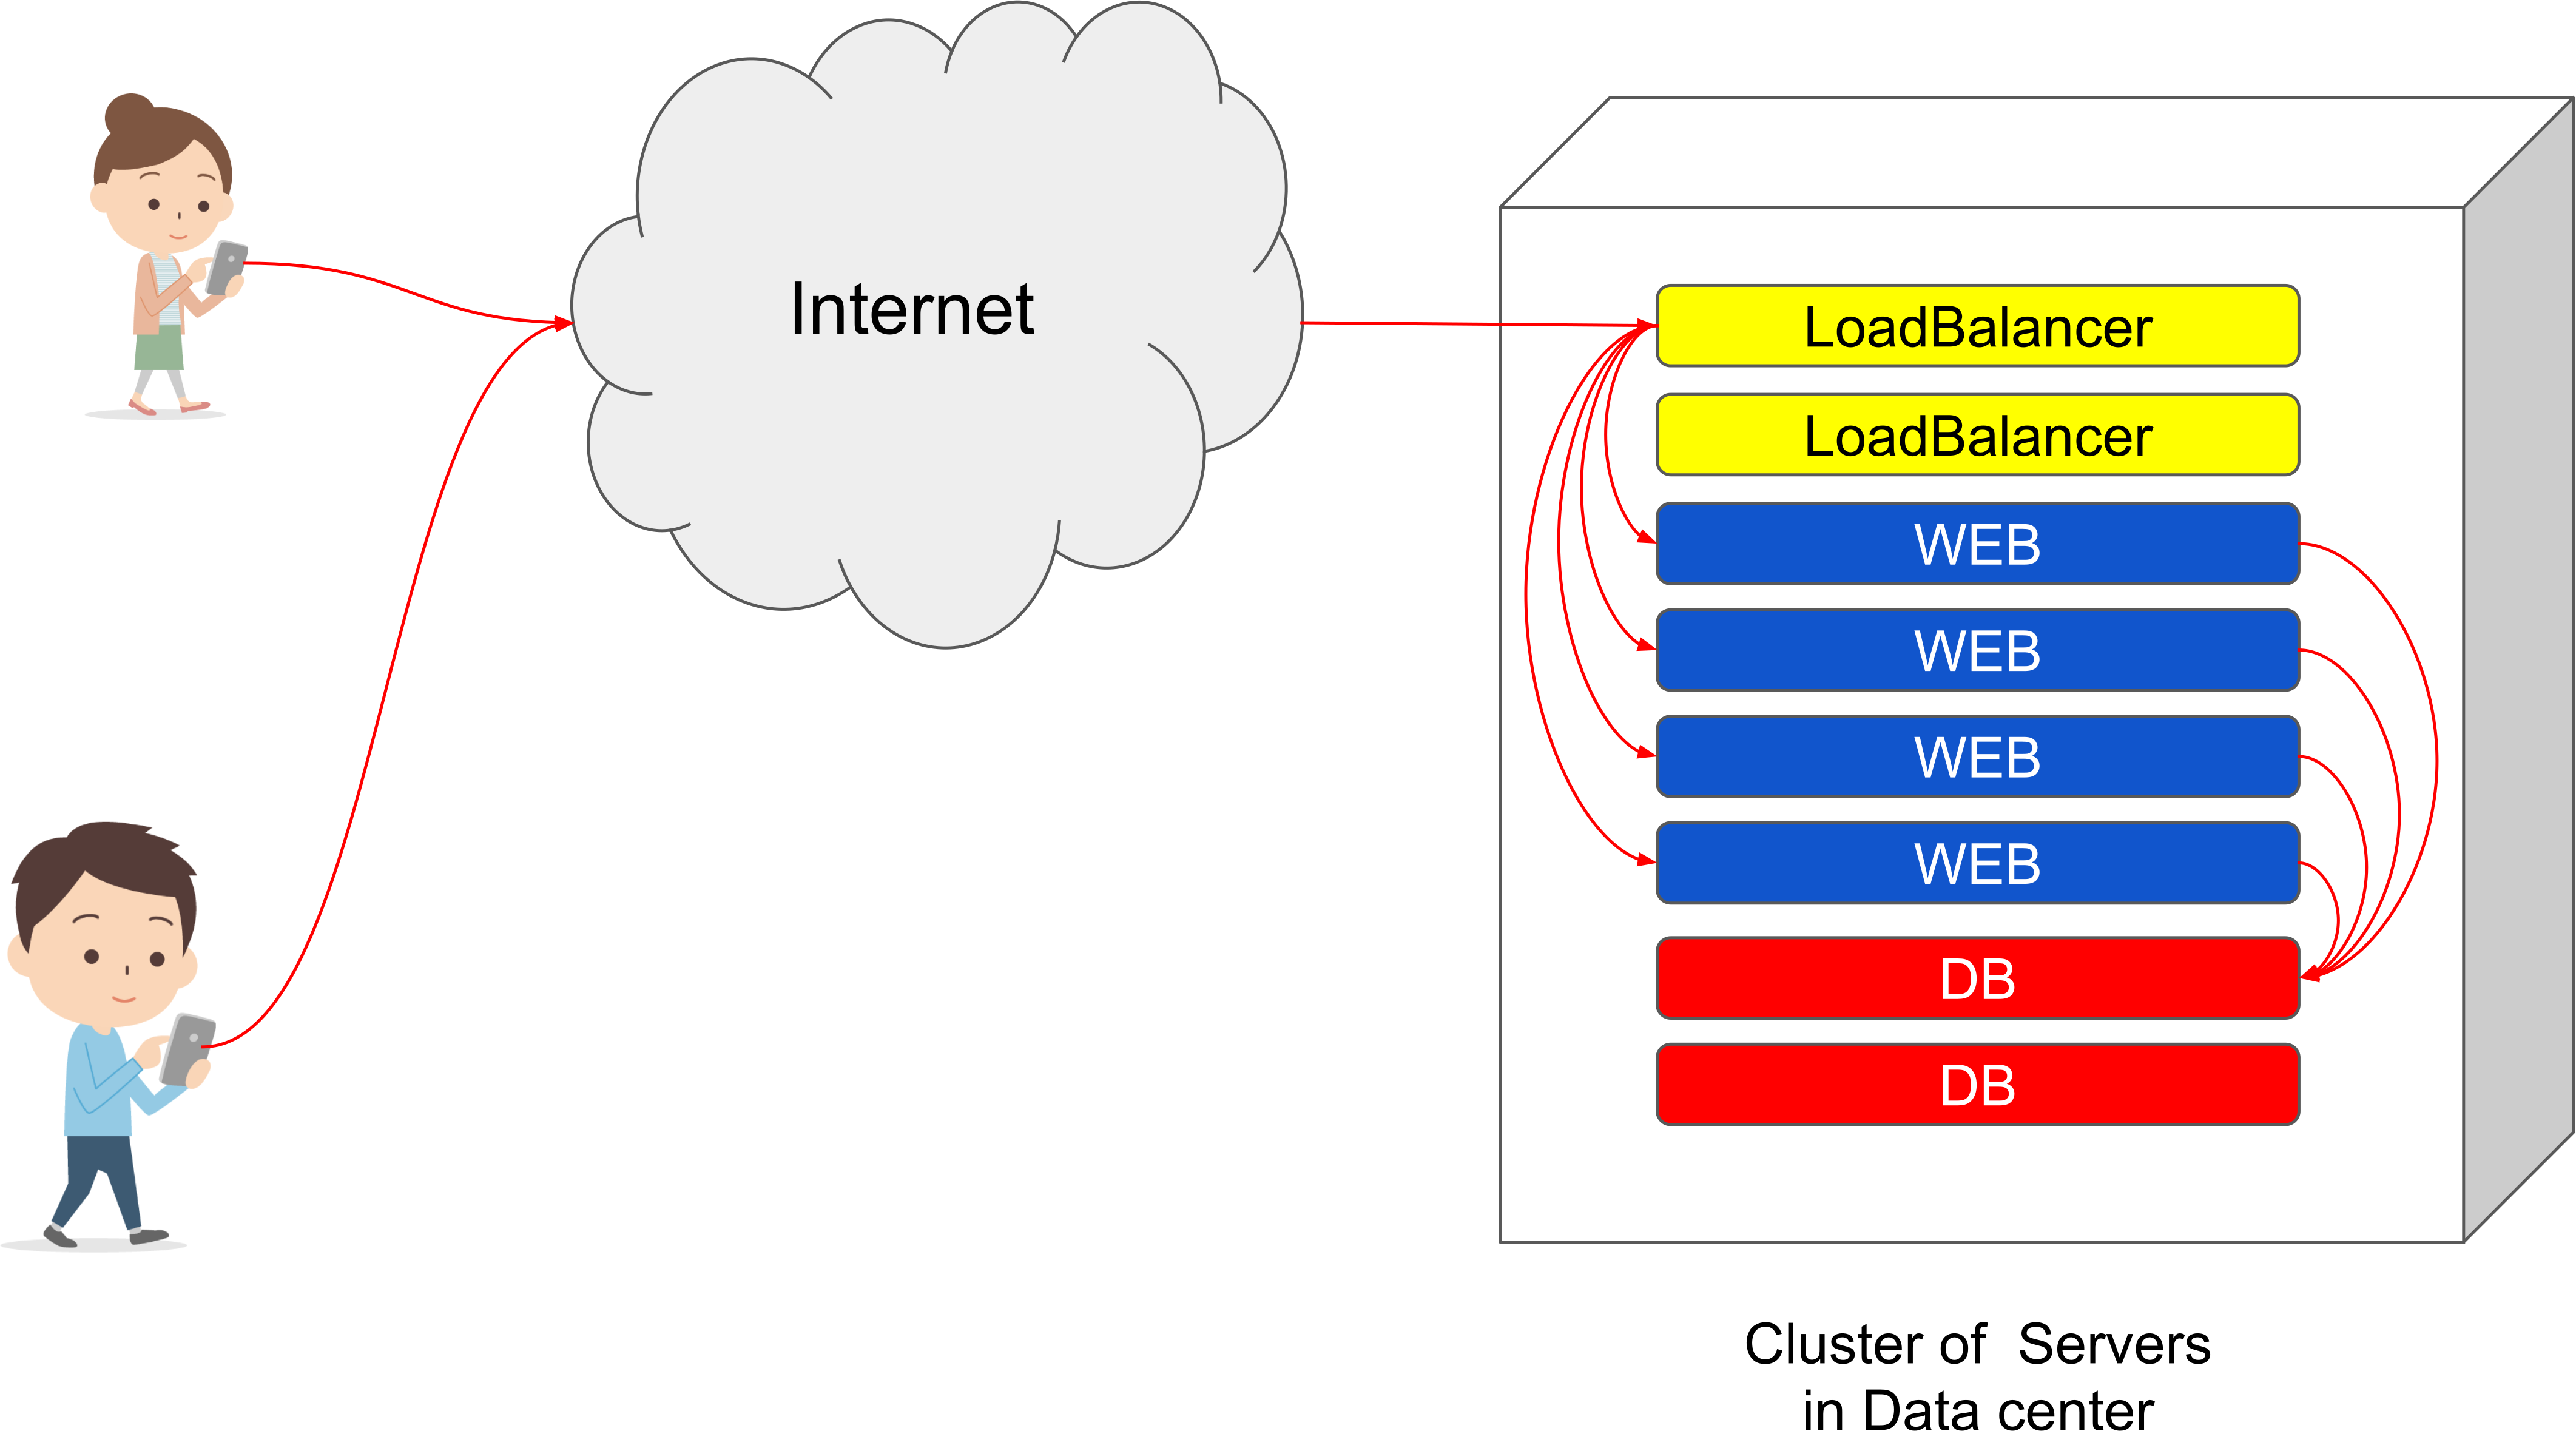
\includegraphics[width=0.8\columnwidth]{Figs/web_cluster.png}
\end{center}
\caption{
An example of web application cluster.
}
\centering\parbox[c]{0.9\columnwidth}{
The load balancers distribute requests from clients to multiple web servers.
The web servers form responses using data retrieved from the database servers and send it back to the clients.
Sometimes the web servers also store and update important data into the database servers.
}
\label{fig:web_cluster}
\end{figure}

A client program on PCs or smartphone sends out requests to servers and the servers respond with data that is requested, using HTTP or HTTPS. 
Servers for web applications are usually computers located in a data center.
In the data center multiple servers cooperate to fulfill the need of the clients.
A group of these servers is often called a web application cluster or a web cluster.
Figure~\ref{fig:web_cluster} shows schematic diagram of an example of a web application cluster.

In this example, there are two load balancers, four web servers and two database(DB) servers that work together to respond to the requests from clients.
The load balancers distribute the requests from clients to multiple web servers.
Then the web servers form responses using data retrieved from the database servers and send it back to the clients.
Sometimes the web servers also store and update important data into the database servers.

\subsection{Migration of web application cluster}

As web applications become an essential part of daily life, an outage of the web application service is getting to be a bigger problem.
If something happens to a web application cluster in a data center, people will not be able to access the necessary information.

For example, if web pages run by local government stops, people will not be able to access the information regarding public service.
If a shopping site run by a company stops, customers can no longer buy products and the revenue of the company will be negatively affected.
Outages of web applications by giant companies can have an even bigger impact.
An outage of Gmail or Google search engine will probably stop most of the business activities around the world.
Service down of Amazon.com affect buyers and many businesses that sell products on its platform.

In order to prevent such outages, preparing another web application cluster in a different location in the case for disasters is very important.
For that purpose, it is desirable if a web application cluster can be easily migrated to a different data center.
Migration of a web application cluster becomes more realistic with the use of Linux container technology, which is explained later.

Migration capability of a web application cluster also has other benefits.
If an e-commerce service is successful in Japan, the company that runs the service might want to start the same service in other country, for examlpe, in Europe.
In this situation, the company probably wants to migrate its web applictation cluster to somewhere in Europe, because, for Europian customers, responses from a web site in Europe is quicker than that from a web site in Japan.

\begin{figure}[h]
\begin{center}
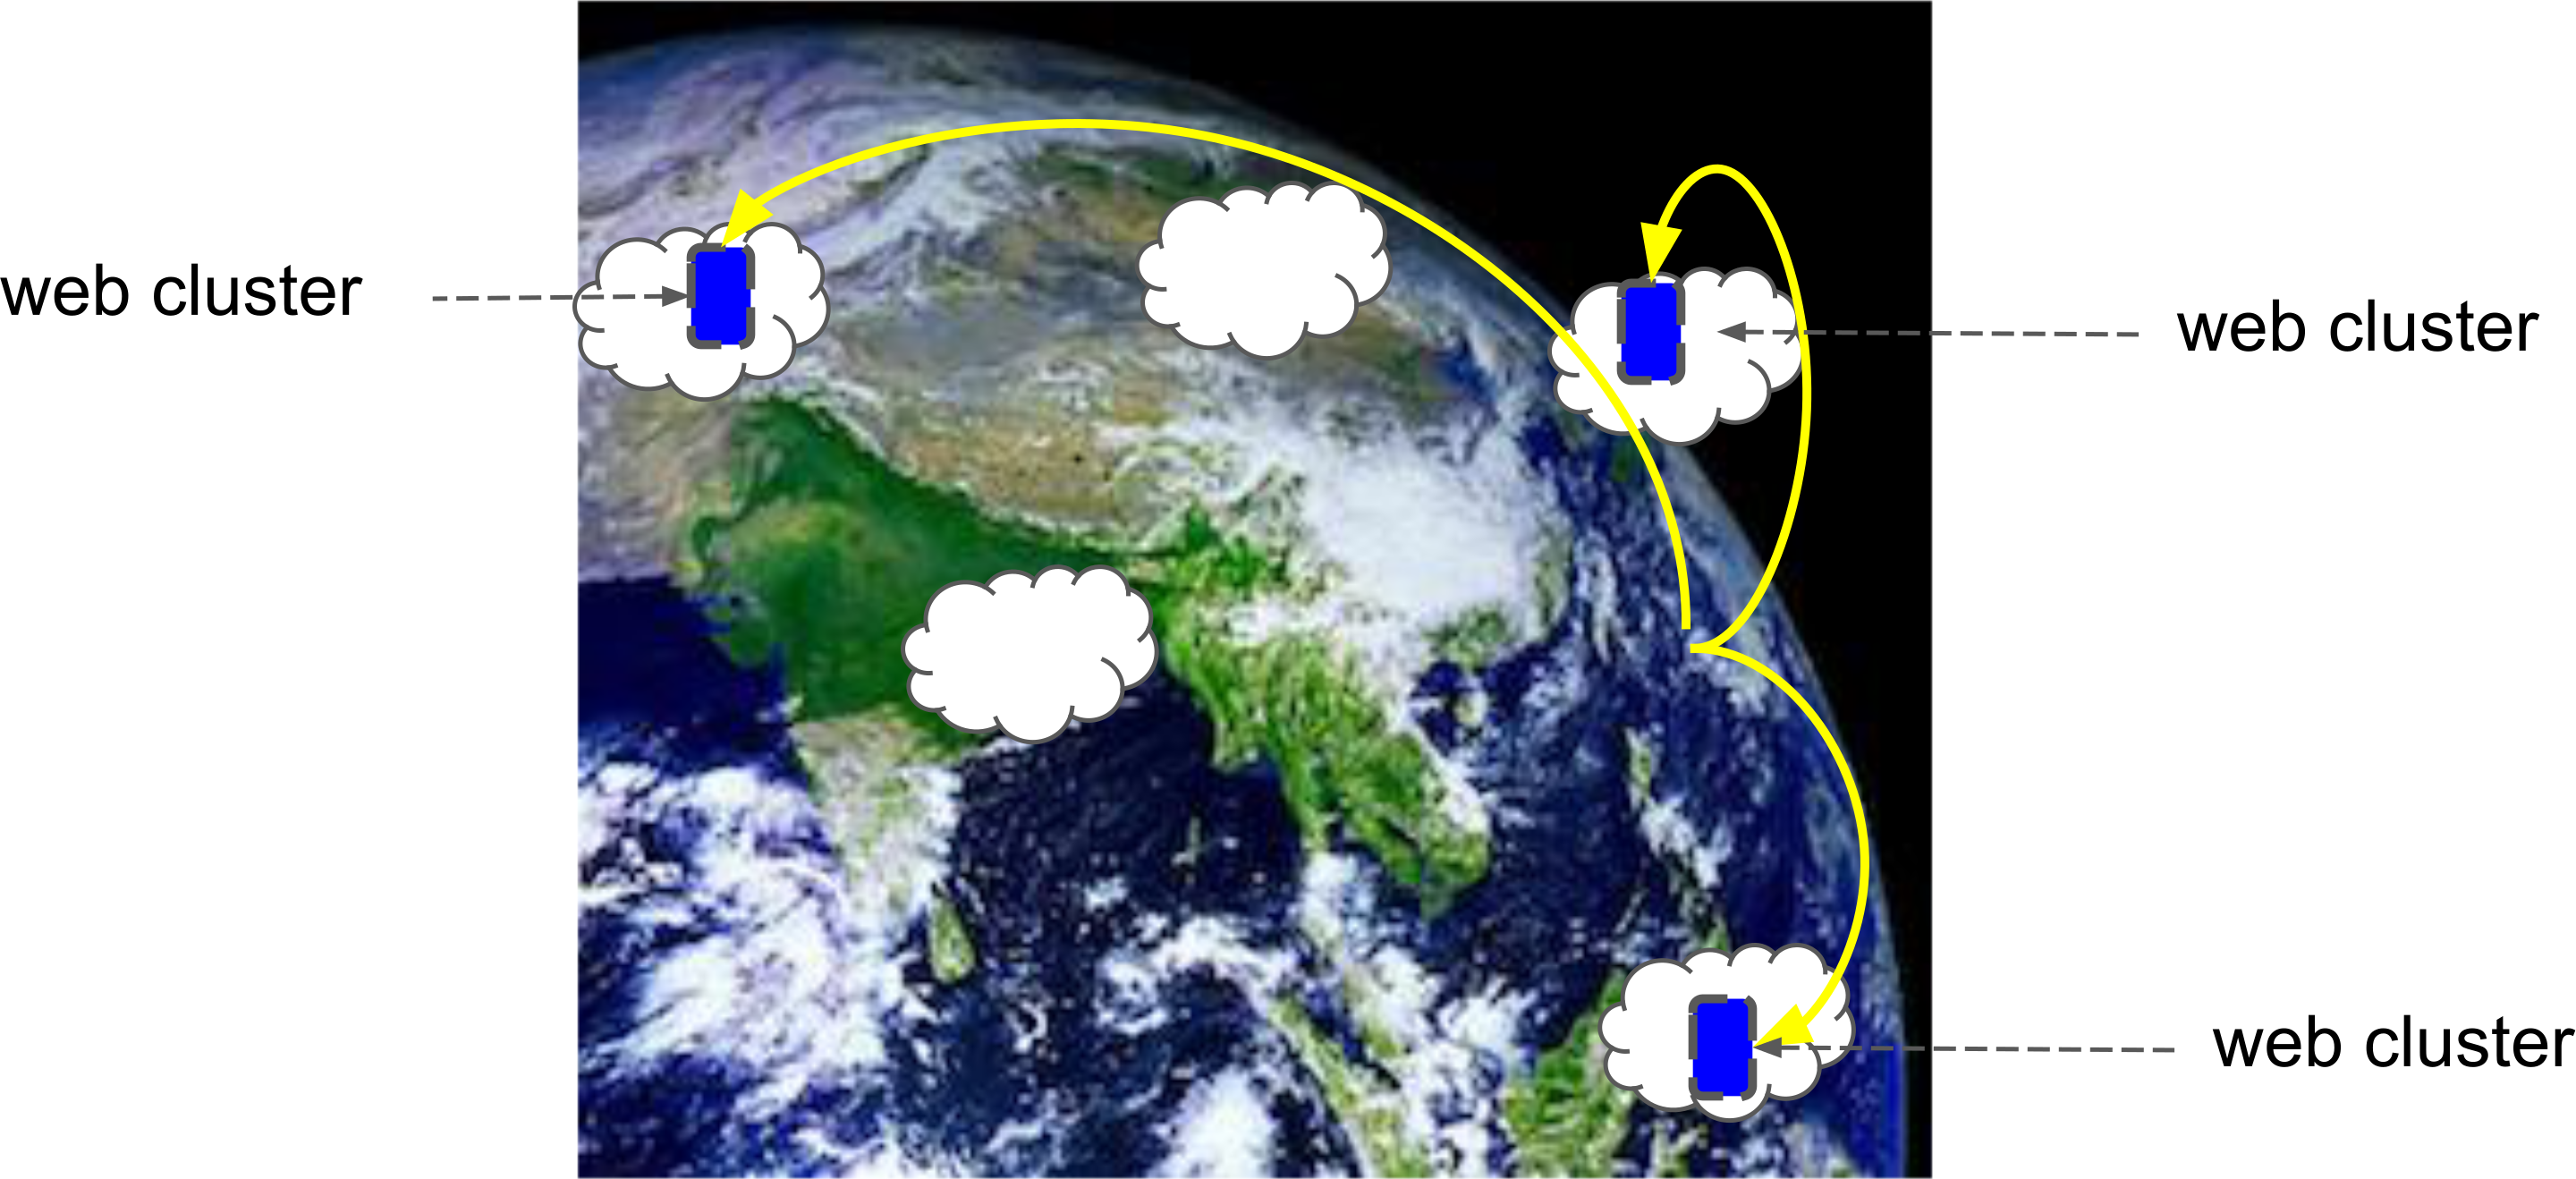
\includegraphics[width=0.7\columnwidth]{Figs/earth}
\end{center}
\caption{
Migration of web application cluster to different locations.
}
\centering\parbox[c]{0.9\columnwidth}{
It is desirable to be able to migrate a web cluster from one place to another with the easiness of on push button.
}
\label{fig:earth}
\end{figure}

Being able to migrate a web application cluster is very important for a variety of purposes, including disaster recovery, cost performance optimizations, meeting legal compliance and shortening the geographical distance to customers.
These are the main concerns for web application providers in e-commerce, gaming, Financial technology(Fintech) and Internet of Things(IoT) field.
Therefore it is important for a web application provider to be able to easily deploy and migrate their web applications among different infrastructure around the world.
The purpose of this research is to propose infrastructures for web application providers, where they can easily deploy their services across the world, regardless of cloud providers or data centers they use.


\subsection{Ideal infrastructure for migration of web application}

\begin{figure}[h]
\begin{center}
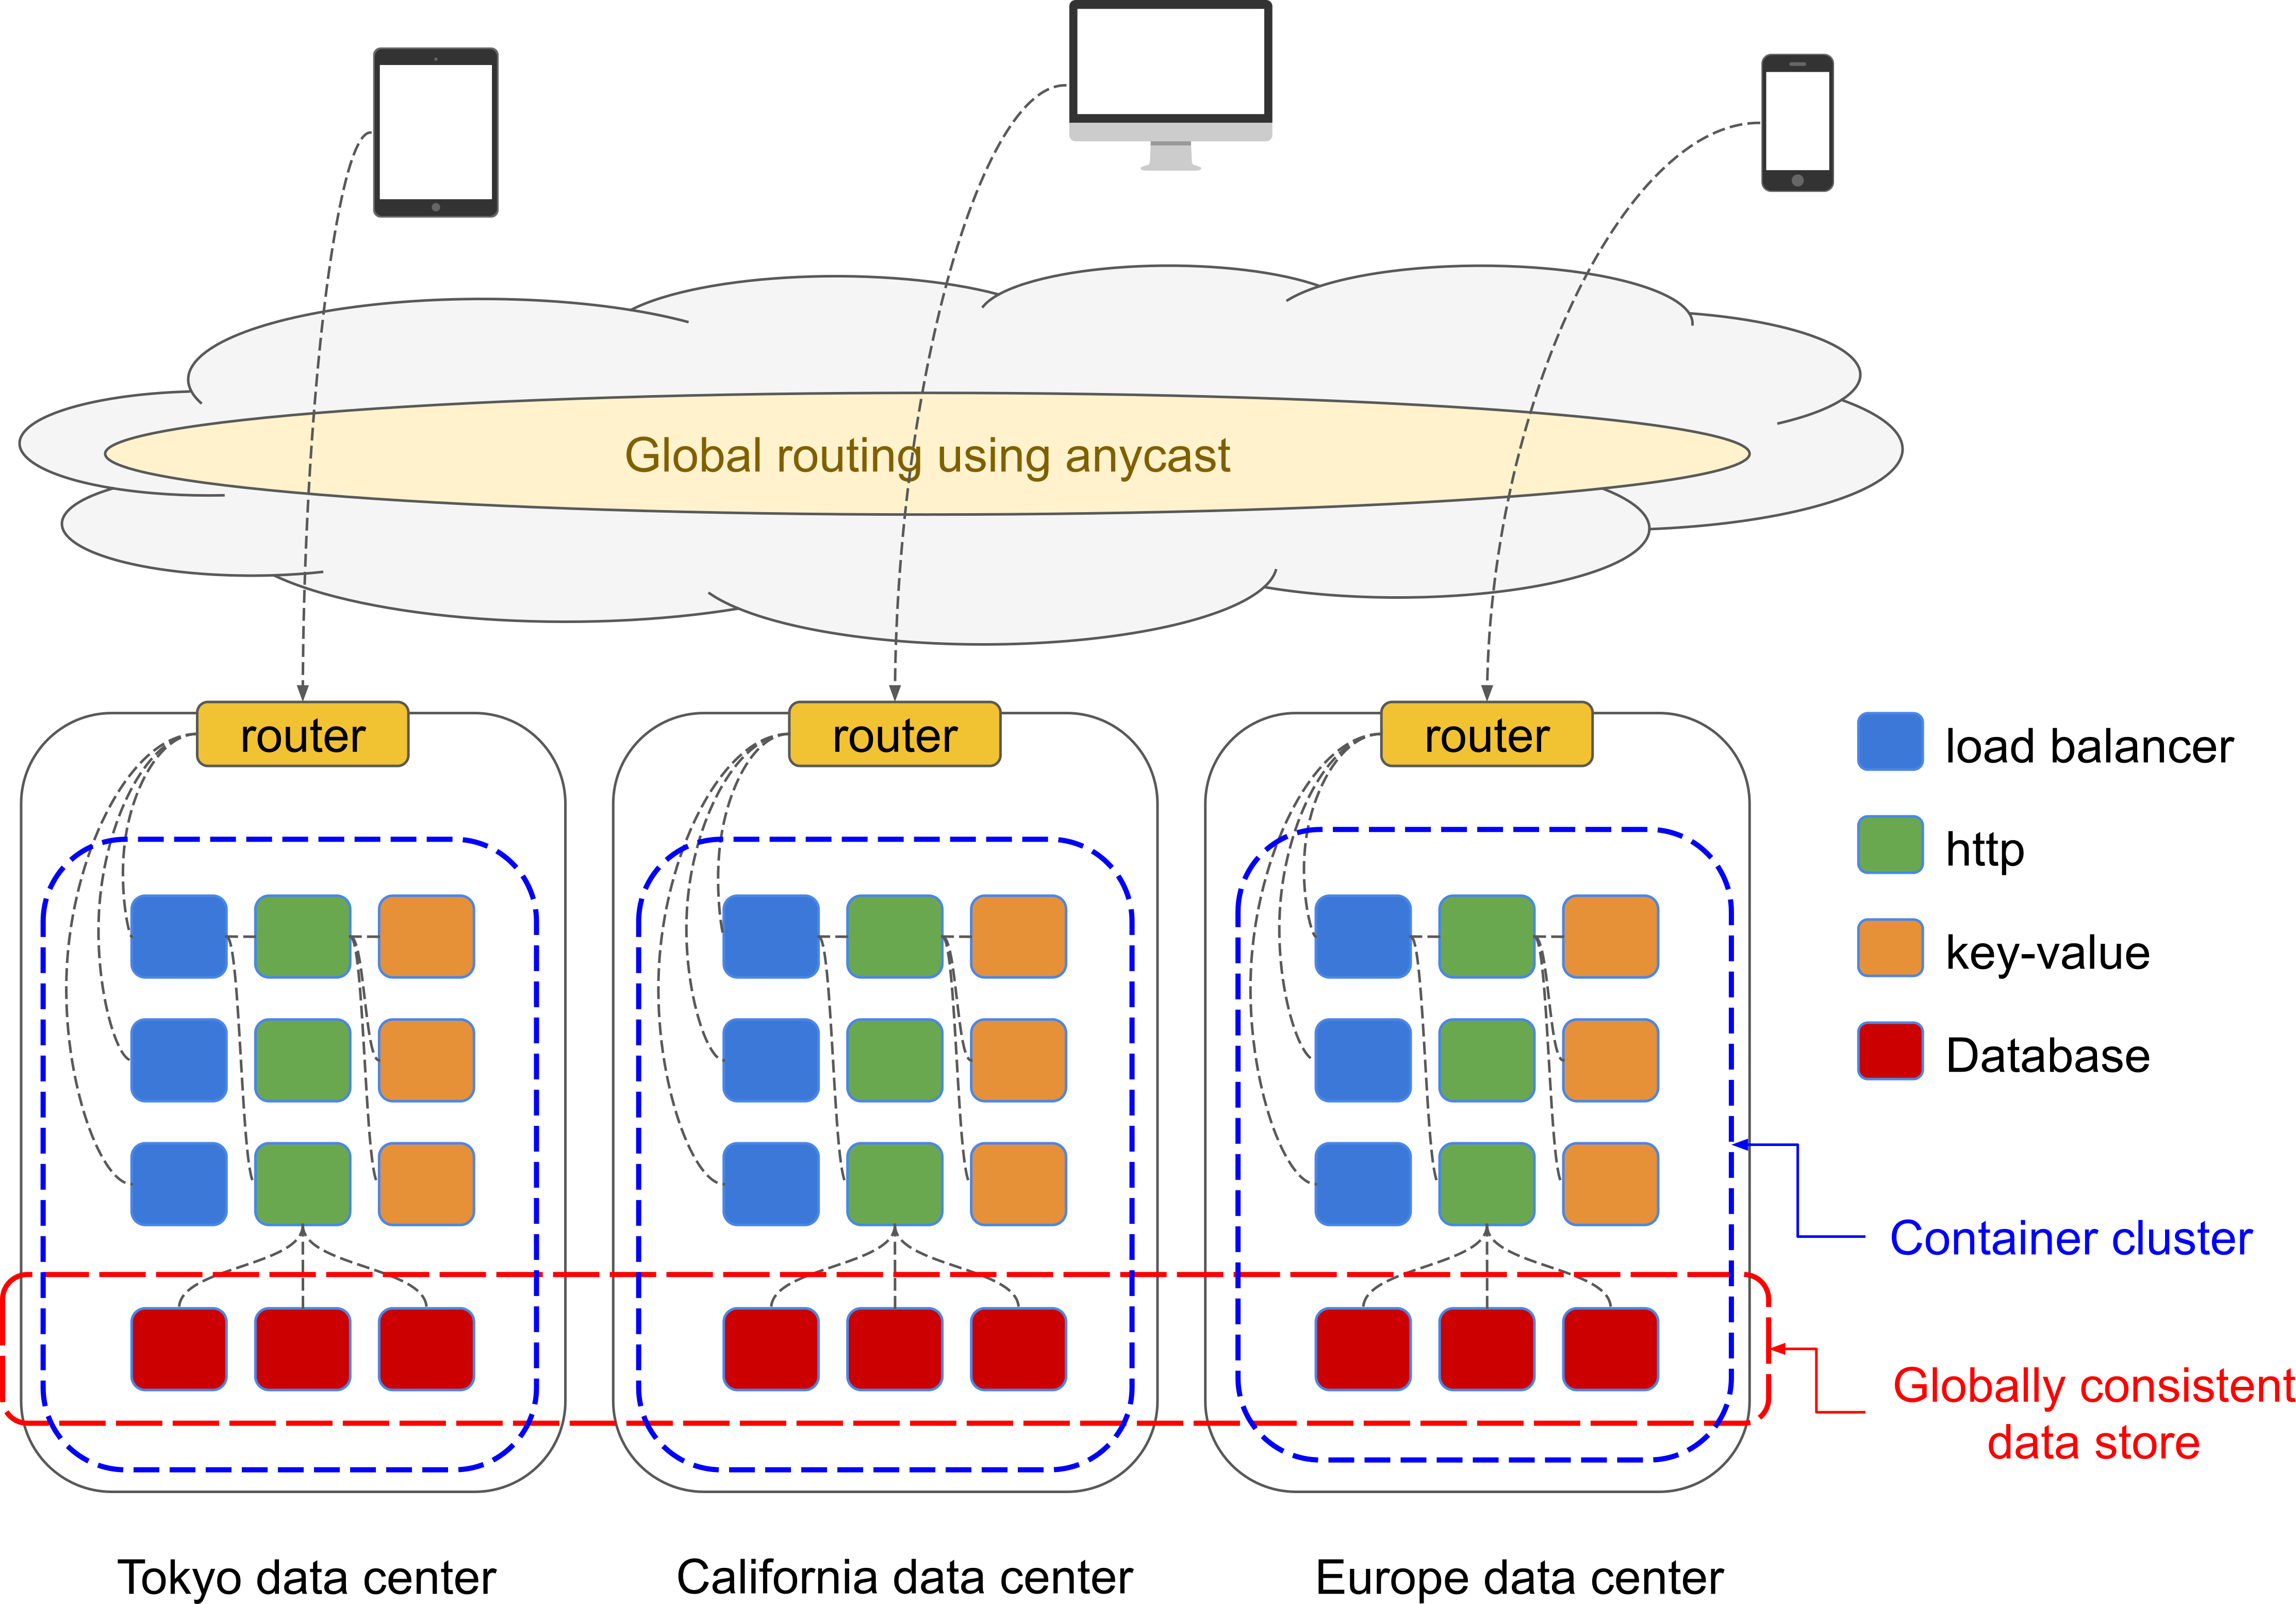
\includegraphics[width=0.9\columnwidth]{Figs/global_container_infrastructure}
\end{center}
\caption{
An ideal global container infrastructure.
}
\centering\parbox[c]{0.9\columnwidth}{
Multiple web application clusters, each of which consisting of a cluster of containers, are deployed in three different data centers as an example.
In each of the data center, container orchestrator manages the container cluster.
Important data are stored in a globally consistent data store.
Access from the client is routed to the closest data center using anycast.
}
\label{fig:global_container_infrastructure}
\end{figure}

In order to realize an easy migration of web applications, an ideal infrastructure probably have the following features;
1) have universal middleware to manage web clusters,
2) store data in globally consistent data storage,
3) route global traffic based on proximity to the client.
%
Figure\ref{fig:global_container_infrastructure} shows an exemplified global container infrastructure having these features.
Container orchestrators launch and manage container clusters.
Important data are stored in globally consistent data storage, which is simillar to the Google spanner\cite{Corbett:2013:SGG:2518037.2491245,Cooper:2013:SGG:2485732.2485756} or CockroachDB\cite{pavlo2016s}.
Traffic is routed to the closest data center using anycast\cite{rfc1546}.

Each of these features is important and research efforts are on-going in many institutions.
In this study, the author focuses on the research regarding container orchestrator as a universal middleware.
%
By realizing global container infrastructure web application providers will be able to deploy their web applications whenever and wherever they want.
Also, they will be able to move their web applications quickly depending on a variety of circumstances, including disaster recovery, cost performance optimization and compliance to government regulations due to trade wars, etc.


\section{Inftastructure for web applications}

\subsection{On-premise data center}

Historically, most of the web application providers purchased servers and installed them in server housing facilities called data centers.
In this type of infrastructure, web application providers typically need to sign a contract with data center company for server housing rack spaces, buy servers and install them in their rented racks by themselves.
They also install OS and software stacks needed to run their web applications in the servers.
Since web application providers place servers in their facilities(either owned or rented), and they are responsible for managing the servers, this type of infrastructure is often called on-premise infrastructure in contrast to Cloud Computing infrastructure.

Preparing data centers, installing the servers and configuring software stacks for web application services often require a considerable amount of time, money and effort.
If web application providers want to expand their services to different countries or if they want to prepare for natural disasters by preparing an additional web application cluster in a different data center, they probably need about the same amount of time, money and effort required to build their original infrastructures.
Therefore migration of web application in this type of infrastructures has always been a daunting task.

\subsection{Cloud computing}

The emergence of Cloud Computing made many things easier for web application providers than before.
Cloud computing utilizes a virtual machine(VM) technology, e.g. KVM, Xen, and VMware.
Cloud computing service providers offer VMs to web application providers with pay-per-use billings.

Figure~\ref{fig:physical_vm_container} compares different type of usages of a single physical server and Figure~\ref{fig:physical_vm_container} (b) shows an example architecture of VM technology.
VMs share a single physical server.
A full OS including Linux kernel is running on top of the virtual machine represented by the hypervisor.
Each VM behaves almost as same as a single physical server.
Since VMs are fractions of a single physical server, server resources are utilized with finer granularities.
Web application providers can start their services with a cluster of VMs, which is smaller than a cluster of physical servers, and hence resulting in lower cost.

Cloud providers generally prepare physical servers and software stacks for VMs before renting it to users, and they also provide an easy to use web user interfaces.
As a result, users only need to click a few buttons on web browsers and wait for a few minutes before obtaining up-and-running VMs.
This simplicity will bring agility to web application providers when they launch their services.
And since computing resources are offered with per-second pay-per-use billings, web application providers can quickly reduce the cost by stopping excessive VMs, when the demand for computing power is scarce.
This was impossible when web application providers purchased physical servers and used them as bare metal servers.
In short, cloud computing brought users agility, flexibility, and cost-effectiveness.

\begin{figure}[h]
\begin{center}
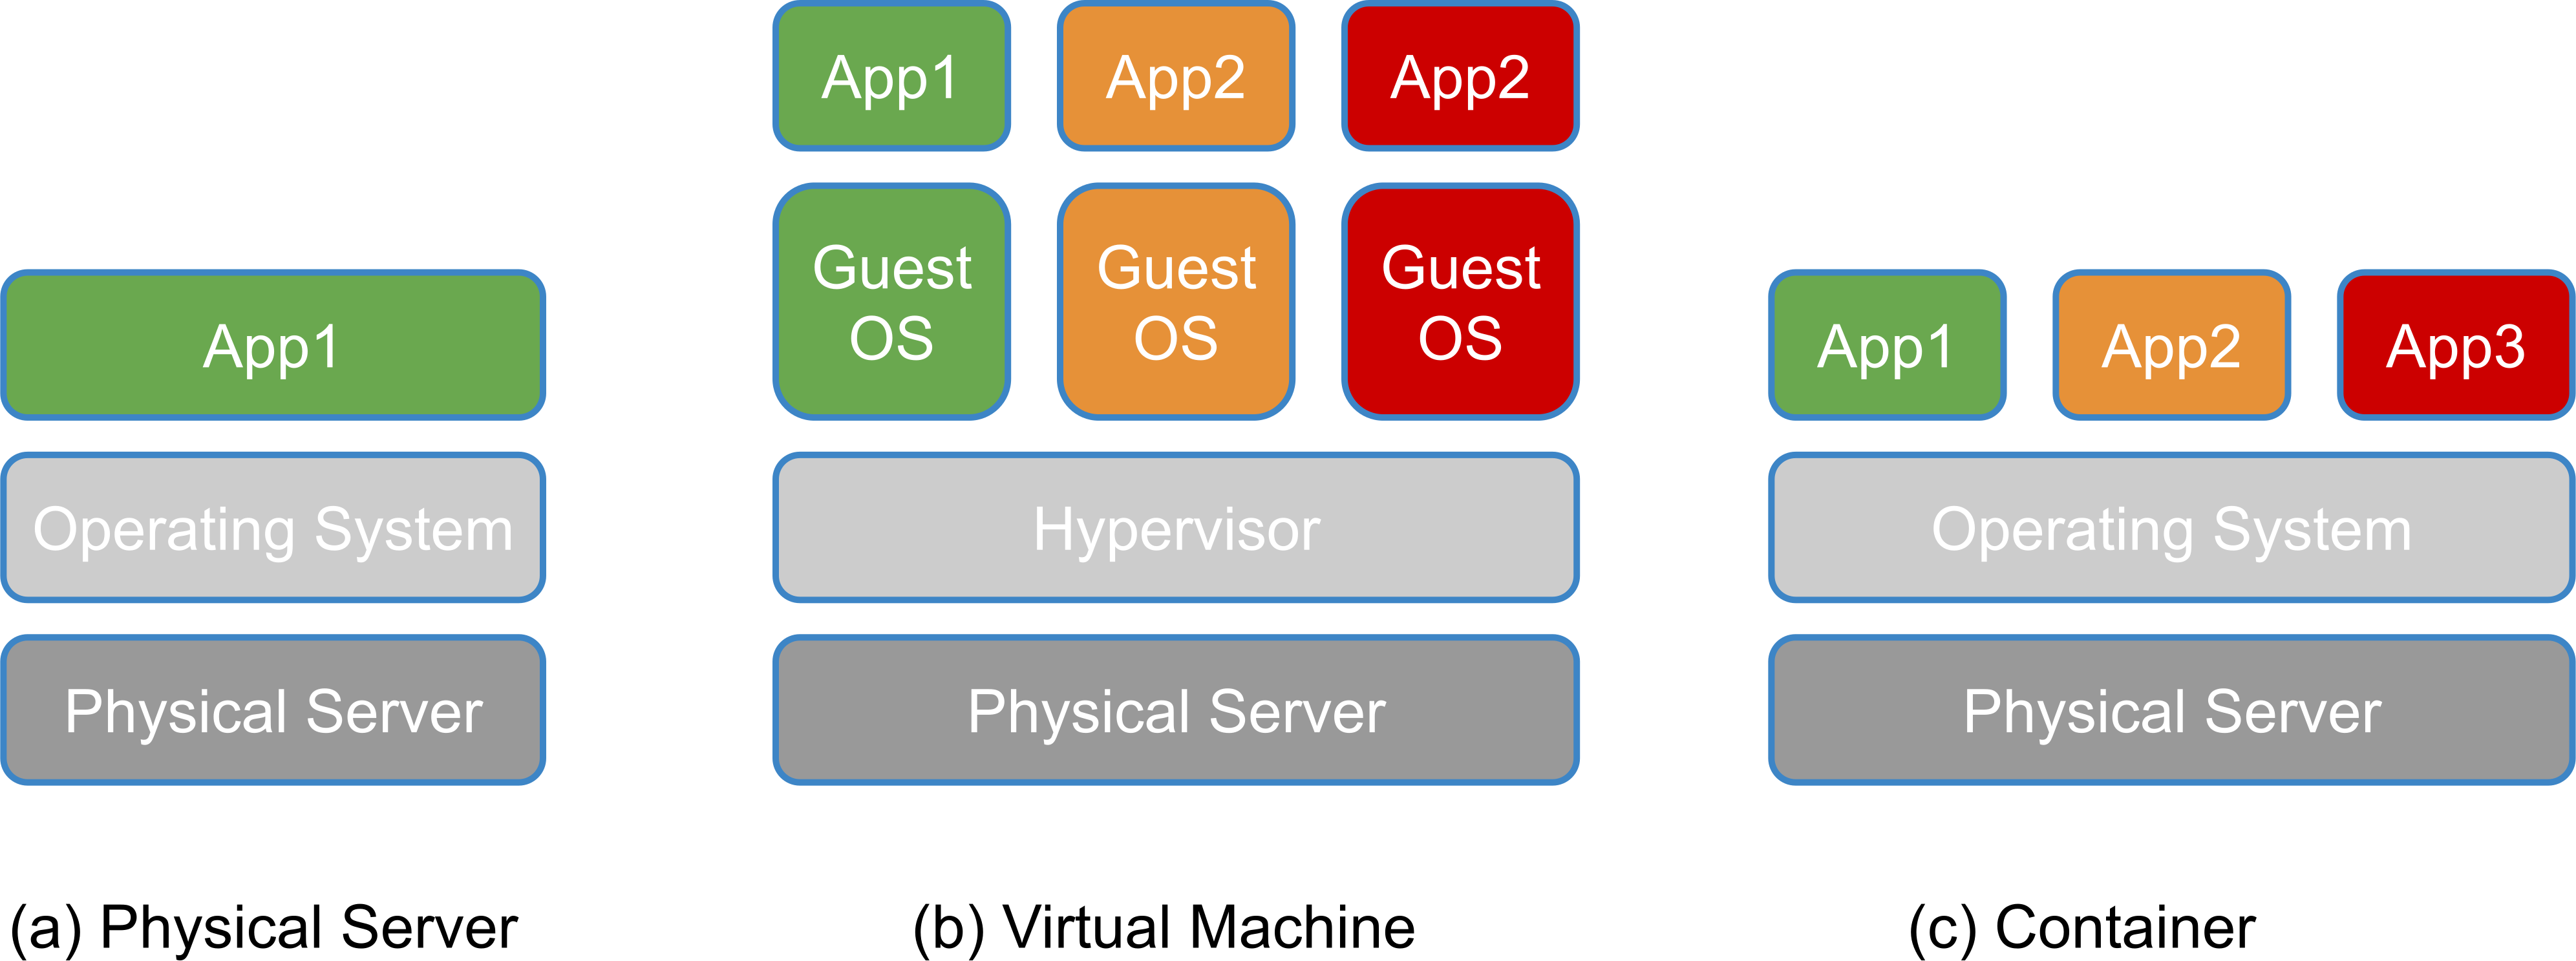
\includegraphics[width=0.8\columnwidth]{Figs/physical_vm_container.png}
\end{center}
\captionsetup{margin=1cm}
\caption{
The difference in physical server usage between (a) Bare Metal servers, (b) Virtual Machine and (c) Container technology.
}

\centering\parbox[c]{0.9\columnwidth}{
(a) Bare Metal servers is a word to describe conventional physical servers in contrast to Virtual Machines.
On top of a Bare Metal server, an operating system and application programs are running.
(b) Virtual Machine technology utilizes physical server hardware and a hypervisor.
The hypervisor provides generic representations of server hardware, which are called virtual machines.
A full operating system and applications are running on each of the virtual machines.
(c) Container technology separates applications by containing them to their respective namespaces.
Applications can not see each other's file systems, networks, users and process IDs unless they belong to the same namespace.
Since container technology merely relies on Linux kernel's namespace function and optionally cgroup, a containerized process does not have any additional overhead compared with a process running on a conventional physical server and operating system.
Container technology can be also utilized on top of virtual machines.
}
\label{fig:physical_vm_container}
\end{figure}

\subsection{Container technology}

More recently, Linux containers\cite{menage2007adding} have come to draw a significant amount of attention.
Figure~\ref{fig:physical_vm_container} (c) shows an example architecture of container technology. 
Linux containers are merely the processes with separate execution environments that are created using the Linux kernel's namespace feature.
The namespace feature can isolate visibility of resources on a single Linux server.

Every process in a container is assigned to a certain namespace, and if two processes belong to different namespaces, they can not see each other's resources. 
Linux kernel implements filesystem namespace, PID namespace, network namespace, user namespace, IPC namespace, and hostname namespace. 
For example, every filesystem namespace can have its own root filesystem, and every network namespace can have its own network devices and IP addresses.
Therefore, it is possible to configure processes as if they were running in different Linux systems by assigning them to different namespaces, although they share kernel and hardware.
While a VM needs to run a full OS on top of a hypervisor and hence imposes extra overhead, a process in Linux container is merely a process with a dedicated namespace and hence imposes no extra overhead.

The Linux container can run on any Linux systems including physical servers and VMs.
Due to the widespread usage of Linux systems, the Linux container can run in most of the cloud infrastructures and on-premise data centers, which is beneficial for migrations.

Several management tools are available for Linux containers, including LXC\cite{noronha2018performance}, systemd-nspawn\cite{jedge2013} and Docker\cite{merkel2014docker}.
These tools assign an appropriate namespace to a process upon the launch of itself and make it look like running in its own virtual Linux system.
For example, container tools restore a file system from an archive file every time a container is launched. 
Container tools also set up separate network interfaces with separate IP addresses in the container's namespace.

The fact that each container has its own file system that is restored from a single archive file brings a significant benefit, i.e. a program binary and shared libraries are always exactly the same regardless of the base infrastructure.
Therefore a process in a container is guaranteed to behave exactly the same manner, even if totally different data centers or cloud providers are used.
This was not easy when there was no container technology.
Because there are many flavors of Linux distributions, and even if the same distribution is used, there was always a chance that a slight difference in a program binary version or library versions could have broken the expected behavior.

In addition to that, containers can have own version of libraries in their respective filesystems, in other words, libraries in any container can be independently updated without influencing other containers.
In conventional technologies, processes on a single server are dependent on common shared libraries, and hence updates of the library sometimes have caused unexpected side effects.
Container tools alleviate these problems by packing necessary libraries into archives. 

Thanks to these benefits container technologies are very attractive for web applications and their migrations.
Considerable efforts in utilizing container technologies for web applications are ongoing.
And to simplify the deployment of a complex web application that consists of interdependent container clusters, several container orchestrators(container management systems)\footnote{The author uses the word 'container orchestrator' and 'container management system' for the same meaning and uses them interchangably} have been in development.

\subsection{Container Orchestrator}

\begin{figure}[h]
\begin{center}
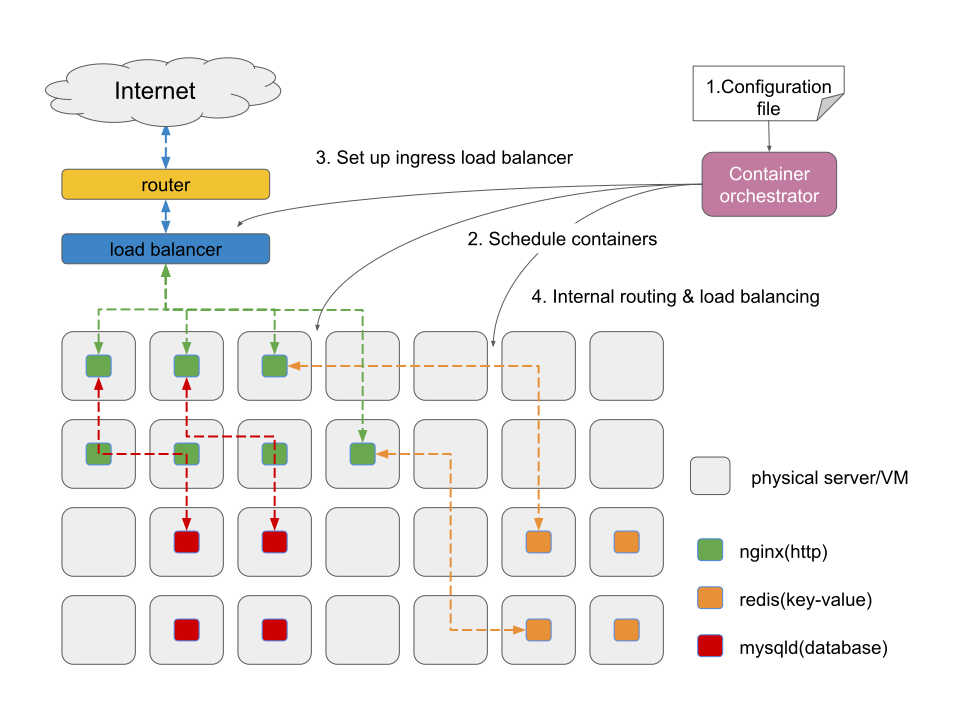
\includegraphics[width=0.9\columnwidth]{Figs/container_management_system}
\end{center}
\caption{
A web application cluster and container orchestrator.
}
\centering\parbox[c]{0.9\columnwidth}{
A web application cluster consists of nginx(http), redis(key-value store) and mysqld(database) is depicted in this figure. 
Each of the component consists of a container cluster.
Container orchestrator recieve configuration file(1), schdule containers(2), set up ingress routing using load balancer(3) and set up internal routing(4).
}
\label{fig:container_management_system}
\end{figure}

A container orchestrator (also called container cluster management system) is a tool to simplify the management of a cluster of containers that are launched on multiple servers.
%
%A container orchestrator is the most important part of the infrastructure for easy migration, not only because it can act as common middleware that hides differences among base infrastructures, but also because it can drastically simplify the deployment of interdependent container clusters.
%
Figure~\ref{fig:container_management_system} shows the important features for the container orchestrator for web applications;
1) {\bf Configuration file:} Orchestrator should manage container clusters based on a configuration file. 
The configuration file must be able to describe container cluster internals and relationships between interdependent container clusters.
2) {\bf Scheduling:} Depending on the configuration file, the orchestrator must be able to pick servers and launch containers on them.
Orchestrator must also maintain the state described in configuration files, for example, the orchestrator may need to maintain the number of running containers.
3) {\bf Ingress routing:} The orchestrator must be able to set up routes for incoming traffic from the internet to multiple containers in a redundant and scalable manner.
4) {\bf Internal routing:} If the web application consists of multiple interdependent container clusters, the orchestrator must be able to set up routes between them in a redundant and scalable manner.

In a configuration file a user can describe how a container cluster should be configured, and also can describe relationships between different clusters.
As a result, a user can launch a web application that consists of interdependent container clusters just by supplying the configuration file to the orchestrator.
For example, a web cluster in Figure~\ref{fig:container_management_system} consists of three different functionalities, namely http server, key-value store, and database.
Each of those consists of a container cluster.
In the configuration file, the relationships between http server cluster, key-value store cluster, and database cluster are specified.
The configuration file also contains how each cluster should be configured, including the number of the containers and resources assigned to them.
Users only need to feed the configuration file to the orchestrator to launch the web application.

Thanks to these features, an orchestrator can be viewed as if it is an Operating System for a server farm in a data center, which not only schedules and launches containers on the server farm but also routes the traffic to the appropriate containers.
By using orchestrators, a user can start a complex web application that consists of multiple interdependent container clusters, on multiple servers in a data center, as easily as starting a single process on a single computer.
As a result, a user can also easily migrate their web applications at his or her convenience.
And migrated web applications are guaranteed to behave exactly the same manner, not only because the same program binary and libraries are used in container, but also because container orchestrators hide difference among the base infrastructures.

Several container orchestrators are available, including Kubernetes, Docker swarm and Mesos/Marathon.
Each of the container orchestrators varies in target applications, and thus has the strength and weaknesses.

\paragraph{Kubernetes}
Kubernetes\cite{burns2016borg} is an open source container orchestrator, originally developed at Google based on their experience of production container orchestrator, Borg\cite{Verma2015}. 
Since Google runs many of large scale web applications, Kubernetes are considered to be best suited to run web applications.

\paragraph{Docker swarm}
Docker Swarm is a container orchestrator built in Docker daemon itself.
Users can execute regular Docker commands, which are then executed by a swarm manager. 
The swarm manager is responsible for controlling the deployment and the life cycle of containers.

\paragraph{Mesos/Marathon}
Mesos\cite{hindman2011mesos} is a common resource sharing layer for different type of applications like Hadoop, MPI jobs, and Spark in a Data Center. 
By using Mesos user does not neet to have dedicated pysical server cluster for each applications.
Marathon is a framework which uses Mesos in order to orchestrate Docker containers.
Because of the broader scope of applications, an out of box Mesos might not be particularly suited for web applications.

\begin{table}[H]
  \centering
  \begin{tabular}{|l|c|c|c|}
    \hline
    & \multicolumn{1}{c|}{Kuberenets} & \multicolumn{1}{c|}{Docker Swarm} & \multicolumn{1}{c|}{Mesos Marathon} \\ \hline
    Config file & Yaml & Yaml & Json  \\ \hline
    Scheduling & Yes &  Yes &  Yes  \\ \hline
    Ingress routing & \begin{tabular}{c} Static\\ Cloud load balancer$^{*}$\end{tabular} & Static & Static \\ \hline
    Internal routing & iptables DNAT & ipvs &  haproxy  \\ \hline
  \end{tabular}
  \caption{Container orchestrator comparison.}
  \centering\parbox[c]{0.9\columnwidth}{
    Important aspects of features as web application infrastructures are compared.
    $^{*}$Support for Cloud load balancer is only avalable in limited infrastructures including GCP, AWS, Azure and Openstack.
  }
  \label{table:orchestrator_comparison}
\end{table}

Table\ref{table:orchestrator_comparison} compares these orchestrators based on necessary features as an infrastructure for web applications.
Although all of these orchestrators mostly satisfy the requirements, they rely on static routing for ingress traffic.
Only Kubernetes has the functionality to manage cloud load balancer so that ingress traffic from the Internet is routed to containers in a redundant and scalable manner, nevertheless, this functionality is applicable only for a few cloud environments.

To the best knowledge of the author, none of the existing container orchestrators has full support for the redundant and scalable ingress routing feature.
The author believes this is an open and important topic for research and development, and therefore intends to pursue it.

\section{Portable software load balancer}

\subsection{Load balancer for container clusters}

\begin{figure}[h]
\begin{center}
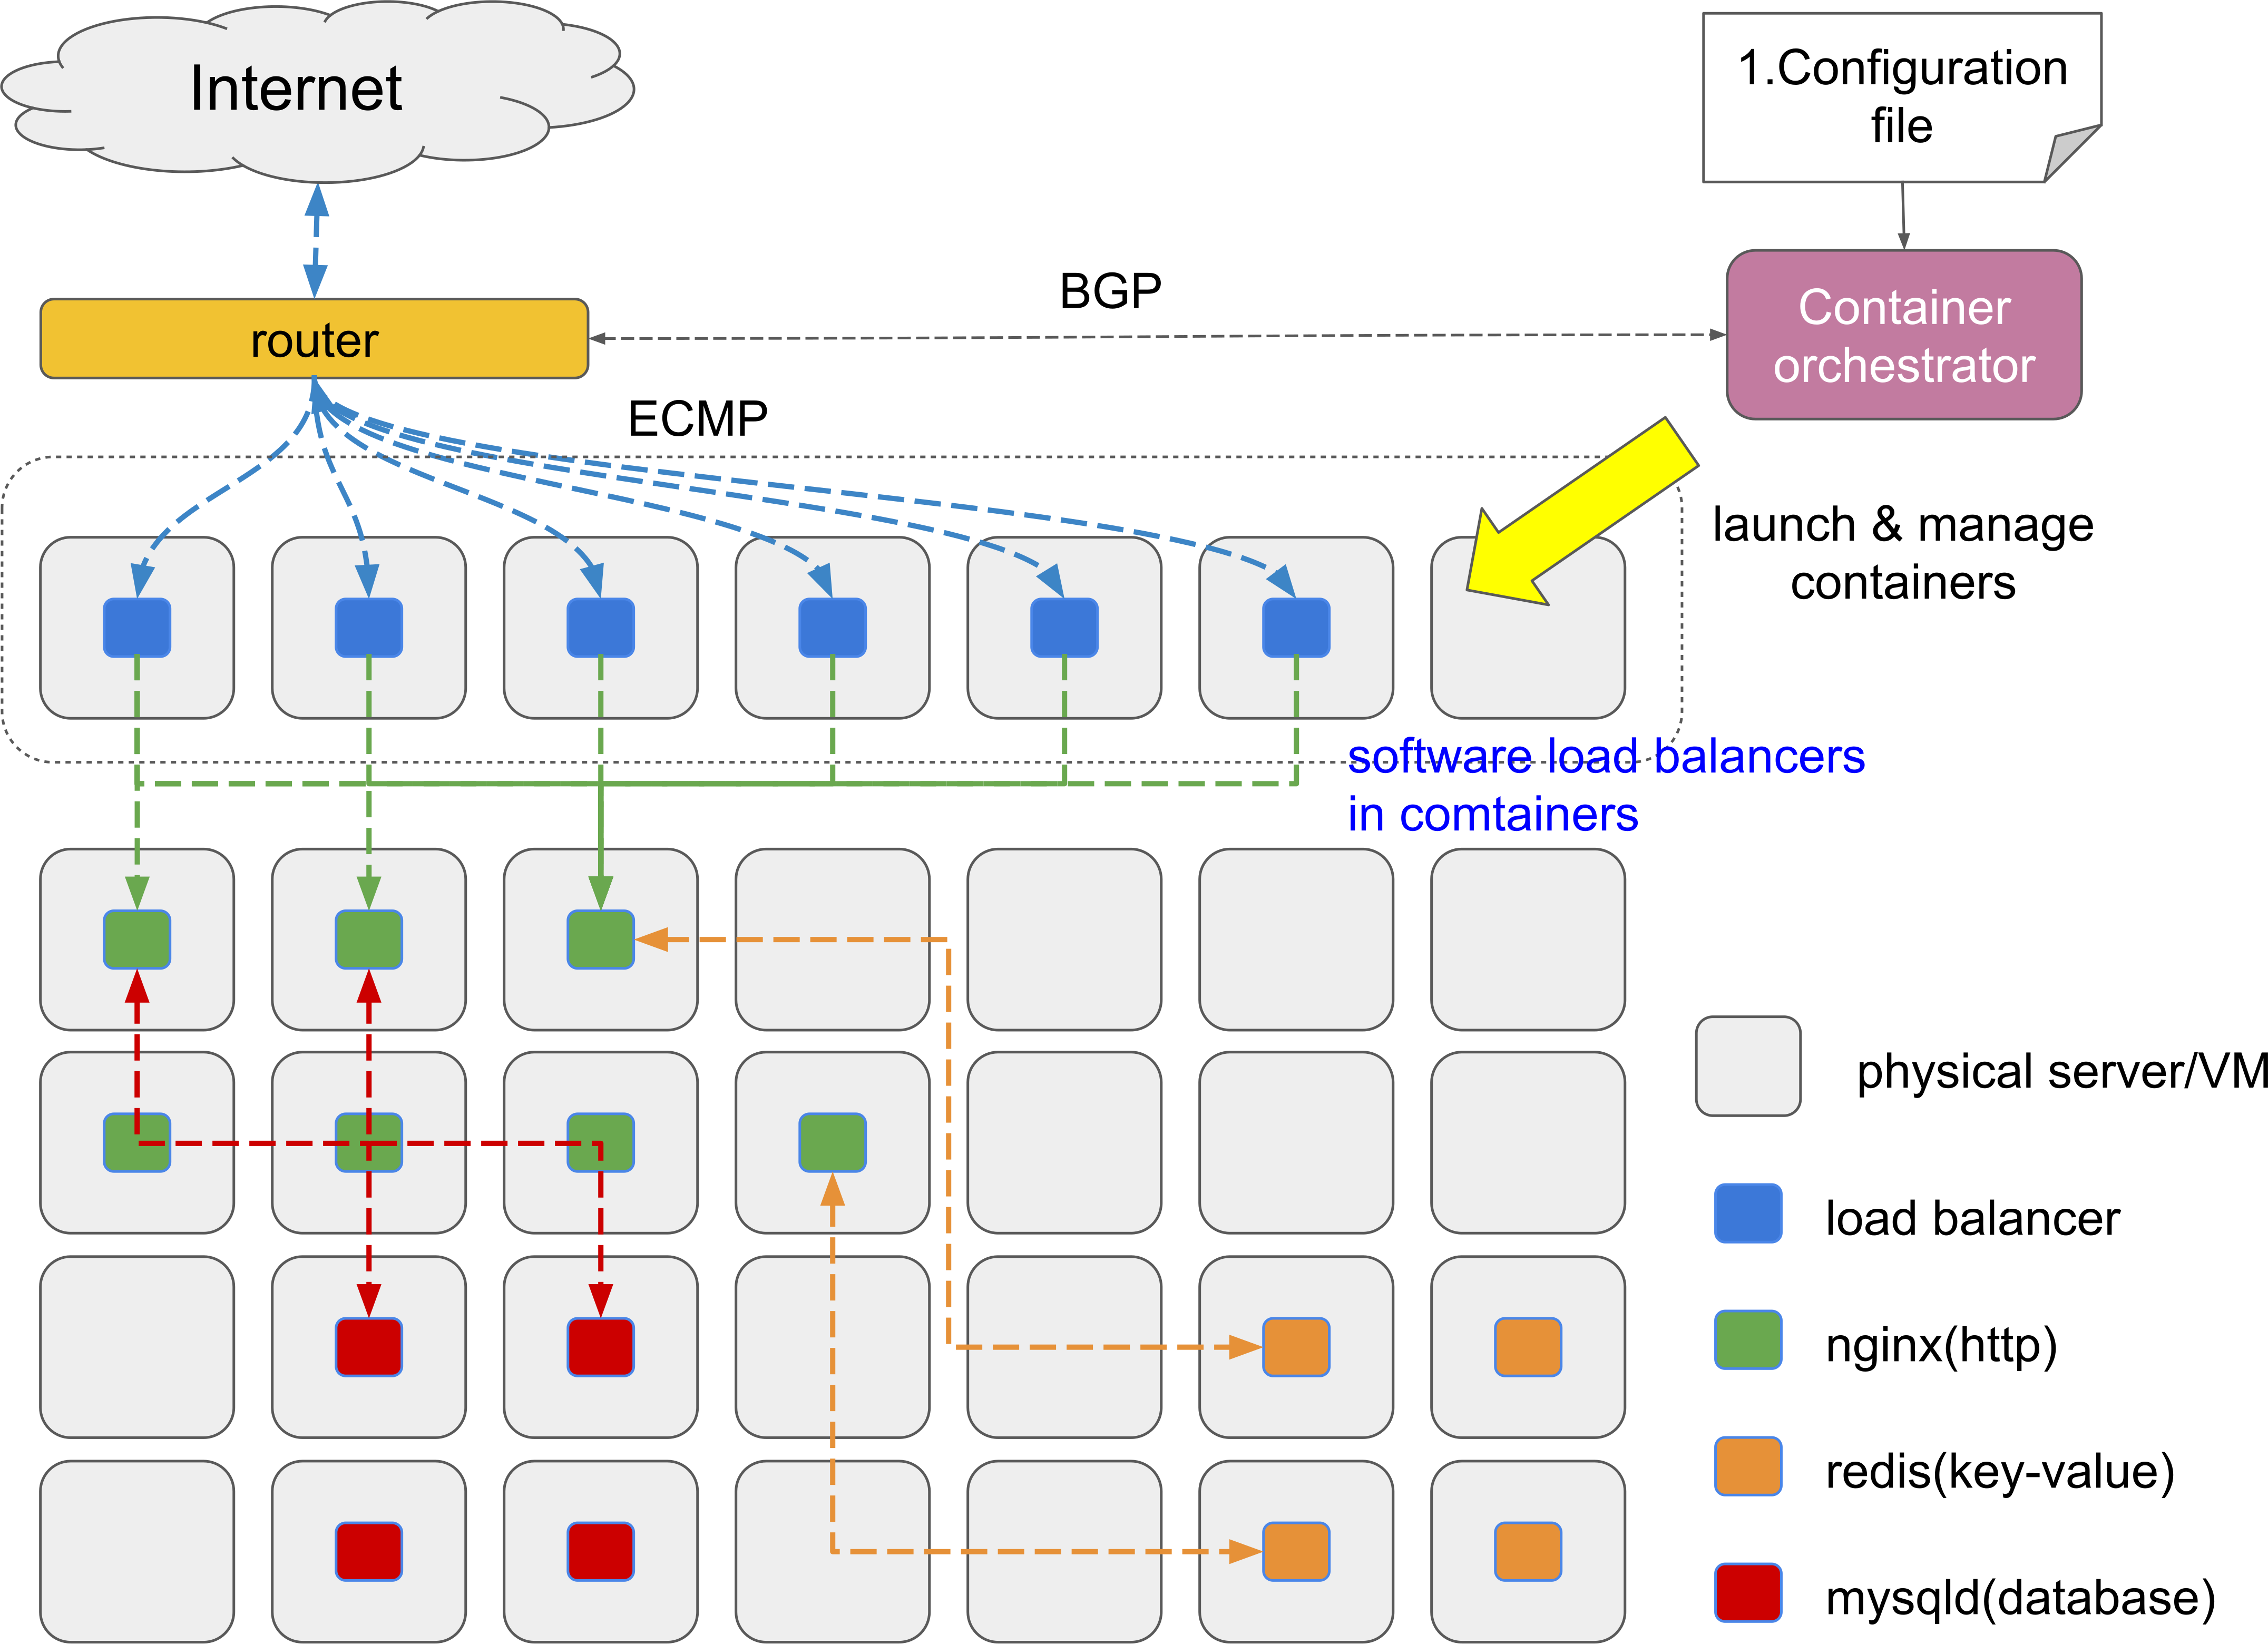
\includegraphics[width=0.9\columnwidth]{Figs/cluster_of_container_loadbalancer}
\end{center}
\caption{
Load balancer for container clusters.
}
\centering\parbox[c]{0.9\columnwidth}{
In order distribute the traffic, container orchestrator launches a cluster of software load balancer containers. 
The container orchestrator also communicates with the upstream router through BGP protocol and the router set up an ECMP routing rule in the routing table.
}
\label{fig:cluster_of_container_loadbalancer}
\end{figure}

The purpose of this research is to investigate a generic way to route the traffic into container clusters in a redundant and scalable manner and thereby to facilitate web application migrations.
In order to bring this into reality, the author proposes a cluster of containerized software load balancers, which is deployed as a part of the web application cluster.

Figure~\ref{fig:cluster_of_container_loadbalancer} shows schematic diagram of an example architecture for such load balancers.
A web application that consists of nginx, redis, and mysqld, each being a cluster of containers, is running in the server farm.
There is also a cluster of software load balancer containers, which is also a part of the web application cluster, running in the same server farm. 
All of the containers are deployed and managed by the container orchestrator.
The orchestrator also communicates with the upstream router using Border Gateway Protocol(BGP), so that the ingress traffic from the Internet is forwarded to the load balancer containers in a redundant and scalable manner using Equal Cost Multi Path(ECMP)\cite{rfc7911} routing table.

Container orchestrators are good at managing a cluster of containers, and they can scale containers, i.e. change the number of containers depending on the needs.
Therefore it seems to be very reasonable to deploy load balancers as a cluster of containers.
In addition to that, by utilizing ECMP routing, redundancy and scalability are accomplished at the same time.
Being able to launch load balancers as a part of web application cluster is very important because users can gain full control of their application cluster.
For example, they can scale the size of the load balancer cluster at their convenience.

The author investigates a cluster of containerized software load balancers for Kubernetes as a test case since Kubernetes seems most appropriate for web application clusters at the moment.
Nevertheless, the author expects general findings of this investigation can be easily applied to the other container orchestrators as well.

\subsection{Problems of Kubernetes}

As is mentioned in the previous section, none of the existing container orchestrators provide full support for automatic set up of ingress traffic routing.
In the case of Kubernetes, the problem is its partial support for external load balancers.
Here the author elaborates on the situation.

Figure~\ref{fig:k8s_intro} shows an exemplified Kubernetes cluster.
A Kubernetes cluster typically consists of a master and nodes. They can be physical servers or VMs.
On the master, daemons that control the Kubernetes cluster are typically deployed. 
These daemons include, apiserver, scheduler, controller-manager and etcd. 
On the nodes, kubelet and proxy are deployed.
The kubelet daemon will run {\it pods}, depending on the PodSpec (pod specification) information obtained from the apiserver on the master.
The proxy daemon will set up iptables DNAT rules that function as the internal load balancer.
A {\em pod} is a group of containers that share the same network namespace and cgroup,
and is the basic execution unit in a Kubernetes cluster.

Thanks to the expressive syntax of the configuration file, Kubernetes allows users to easily launch complex web applications that consist of multiple interdependent container clusters as if they were launching a single application program.
It also allows users to modify the state of their container clusters, just by modifying the configuration file.
Kubernetes always keeps the status of containers to match its desired state, which is written in the configuration file.

When a service is created, the master schedules where to run {\em pods}, and kubelets on the nodes launch them accordingly.
At the same time, the master sends out requests to cloud provider's API endpoints, asking them to set up external cloud load balancers that distribute ingress traffic to every node in the Kubernetes cluster.
The proxy daemon on the nodes also setup iptables DNAT\cite{MartinA.Brown2017} rules. 
The Ingress traffic will then be evenly distributed by the cloud load balancer to all of the existing nodes, 
after which it will be distributed again by the DNAT rules on the nodes to the designated {\em pods}. 
The returning packets follows the exact same route as the incoming ones.

\begin{figure}[h]
  \centering
  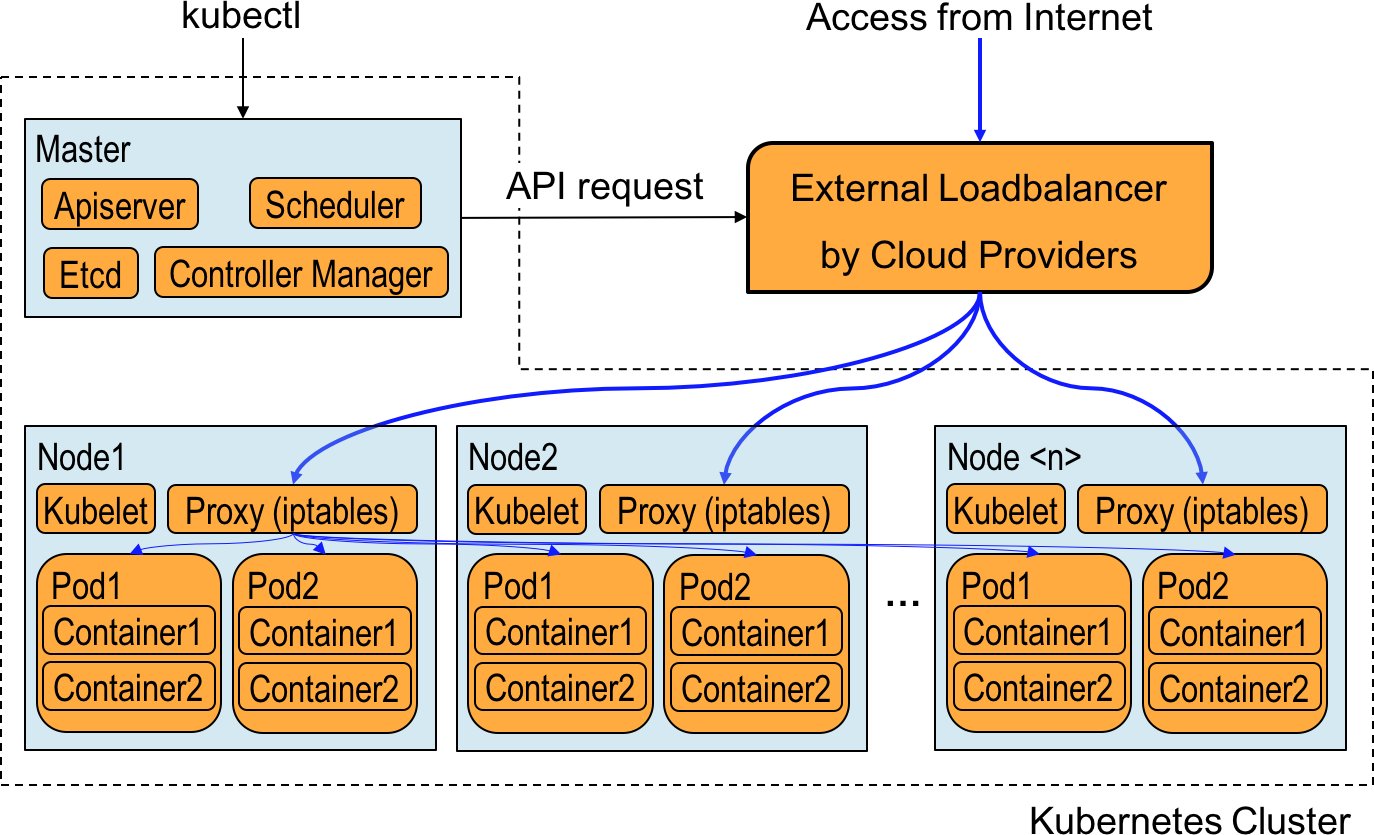
\includegraphics[width=0.8\columnwidth]{Figs/K8sConventional}
  \label{fig:k8s_intro}
  
  \centering
  
  \begin{minipage}{0.9\columnwidth}
    \caption[Architecture of Kubernetes clusters]
            {
              Architecture of Kubernetes clusters.
              A Kubernetes cluster typically consists of a master and nodes, which can be physical servers or VMs.
              On the master, daemons that control the Kubernetes cluster are typically deployed. 
              On the nodes,  daemons that control contair and the internal routing are typically deployed.
              Kubernetes depends on external load balancer to route ingress traffic from the internet into the container cluster.
              However, it seems impractical to support all of the existing load balancers.
            }
  \end{minipage}
  
\end{figure}

Load balancers are often used to distribute high volume traffic from the Internet to thousands of web servers.
They are implemented as dedicated hardware or as software on commodity hardware.
Major cloud providers have developed software load balancers\cite{eisenbud2016maglev,patel2013ananta} dedicated for their infrastructures.
For on-premise data centers, there are a variety of proprietary hardware load balancers.

Kubernets utilizes load balancers to route ingress traffic into the Kubernetes cluster in a redundant and scalable manner. 
Although software load balancers for cloud infrastructure have APIs, through which Kubernetes can control the behavior, most of the proprietary hardware load balancers do not have such APIs.

In environments where there are supported load balancers, namely cloud environments including Google Cloud Platform (GCP), Amazon Web Applications (AWS), or Openstack, Kubernetes can automatically set up the route for the ingress traffic upon the launch of a web application.
The cloud load balancers will distribute ingress traffic to every node(physical servers or VMs) that might host containers.
Once the traffic reaches the nodes, Kubernetes nicely route them to containers using iptables Destination Network Address Translation(DNAT) based internal load balancer.

However, in environments where there are no supported load balancers, Kubernetes fails to automatically set up the route for ingress traffic.
This problem often happens in on-premise data centers,  since there are many proprietary load balancers that do not even have AIPs.
In such cases Kubernetes expects users to manually set up a route for the ingress traffic, which generally lacks redundancy and scalabilities.
Kubernetes fails to provide uniformity that is essential for easy deployment and migration of complex web applications.

Other container orchestrators, e.g. Docker swarm or Mesos/Marathon, do not even have partial support for load balancers and expect users to manually set up the route for ingress traffic.
Therefore this is a generic problem that current container cluster orchestrators possess.

\subsection{Proposed solution}


In order to alleviate this problem, the author proposes a portable and scalable software load balancer that can be used in any environment where there is no load balancer supported by container orchestrators, as a part of web application cluster, as is shown in the Figure~\ref{fig:cluster_of_container_loadbalancer}.
The load balancer should be able to periodically acquire information regarding the running containers, thus always update appropriate balancing rules to existing containers.
Also, the orchestrater should be able to update the routes to existing load balancer contains in the upstream router.
By using a proposed load balancer, users no longer need to manually adjust their services to the base infrastructures.
The route for ingress traffic is automatically set up in a redundant and scalable manner, every time users launch their web application clusters which include a cluster of software load balancer containers.

As a proof of concept the author implements the proposed software load balancer that works well with Kubernetes using following technologies;
1) To make the load balancer runnable in any environment, Linux kernel's Internet Protocol Virtual Server (ipvs)\cite{Zhang2000} is containerized using Docker\cite{merkel2014docker}. 
2) To make the load balancer redundant and scalable, the author makes it capable of updating the routing table of upstream router with Equal Cost Multi-Path(ECMP) routes\cite{al2008scalable} using Border Gateway Protocol(BGP), which is a standard routing protocol.
3) The author also extends the research into implementing the novel load balancer using eXpress Data Plane(XDP) technology\cite{bertin2017xdp} to enhance the performance level to meet the need for 10Gbps network speed.

\subsection{Contribution}

Contributions of this paper can be summarized as follows:
1) The author addresses the problem of ingress traffic routing that is generic to container orchestrators and proposes software load balancer suitable for container environment.
This is one of the most important problems for container orchestrators because without solving this problem migration of a web application will never be easy.
2) The author builds a proof of concept load balancers using OSS, which means that anyone can test drive the proposed load balancers and use them in production for free.
3) The author provides quantitative performance analysis to see the feasibility of proposed load balancer architecture in the 1Gbps network.
4) The author clarifies the remaining problems for future improvement in the 10Gbps network and explores other technology to be used in faster networks.

The outcome of this study will benefit users who want to deploy their web applications on any cloud provider where no scalable load balancer is provided, to achieve high scalability.
Moreover, the result of our study will potentially benefit users who want to use a group of different cloud providers and on-premise data centers across the globe seamlessly.
In other words, users will become being able to deploy a complex web application on aggregated computing resources on the earth, as if they were starting a single process on a single computer.

\section{Outline}

The rest of the paper is organized as follows.
Chapter \ref{chapter:related} and Chapter \ref{chapter:background} provides related works and the background information necessary to understand following chapters.

Chapter~\ref{chapter:Architecture and Implementation} provides discussion of load balancer architecture suitable for container clusters.
First the author discusses problems of conventions architecture in Section~\ref{Problem of Conventional Architecture}.
Then the author proposes a portable software load balancer in container in Section~\ref{Load balancer in container}
After that the author discusses redundancy architecture using ECMP in Section~\ref{Redundancy with ECMP}. 
Chapter~\ref{chapter:Architecture and Implementation} also presents implementation of the proof of the concept system for the proposed load balancer architecture in detail.
First overall architecure is explained in Section~\ref{sec:poc}.
Then ipvs containerization is explained in detail in Section~\ref{sec:ipvs}.
Finally implementation of BGP software container is explained in Section~\ref{sec:bgp}.

Chapter \ref{chapter:portablelb} discusses portability and performance levels of the proposed load balancer in 1 Gbps network environment.
Chapter \ref{chapter:redundancy} discusses the redundancy and scalability of the proposed load balancers.
Chapter \ref{chapter:performance} present the performance levels of the proposed load balancer in 10 Gbps network environment and discuss the method to improve the performance of a software load balancer.
Chapter \ref{chapter:futurework} discusses the limitation and the future work of this study,
which is followed by a conclusion of this work in Chapter \ref{Conclusions}.





